% QTCNN for cross-sectional equity ranking -- manuscript skeleton
% Build: latexmk -pdf main.tex
\documentclass[11pt,a4paper]{article}

\usepackage[utf8]{inputenc}
\usepackage[T1]{fontenc}
\usepackage{amsmath,amssymb}
\usepackage{booktabs}
\usepackage{graphicx}
\usepackage{siunitx}
\usepackage{xurl}
\usepackage[hidelinks]{hyperref}
\usepackage[margin=2.5cm]{geometry}
\usepackage{natbib}
\usepackage{subcaption}
\providecommand{\ket}[1]{\left|#1\right\rangle}
\providecommand{\bra}[1]{\left\langle#1\right|}

\graphicspath{{figures/}}
\sisetup{detect-weight=true,detect-inline-weight=math}

\title{Trained, Frozen, or Absent:\\
Identifying What a Quantum Layer Contributes to\\
Cross-Sectional Equity Ranking}

\author{Chi-Sheng Chen$^{1,*}$ \qquad En-Jui Kuo$^{2}$\\[4pt]
{\small $^{1}$Beth Israel Deaconess Medical Center \& Harvard Medical School, Boston, MA 02115, USA}\\
{\small $^{2}$Department of Electrophysics, National Yang Ming Chiao Tung University, Hsinchu 30010, Taiwan}\\
{\small $^{*}$Corresponding author: m50816m50816@gmail.com}}
\date{}

\begin{document}
\maketitle

\begin{abstract}
Hybrid quantum--classical models are increasingly proposed for financial
prediction, but the reported gains are rarely separated from the classical
components they are wrapped in, or are measured on windows too short to
resolve them. We study a hybrid quantum temporal convolutional
network for daily cross-sectional ranking of \num{2000} Tokyo Stock Exchange
equities under a protocol built to make the quantum contribution identifiable:
five conditions (trained circuit, frozen circuit, parameter-matched classical
surrogate, no circuit, circuit only) trained through one code path; four
rolling-origin walk-forward folds with an embargo and five seeds; annualised
metrics with stationary-bootstrap intervals, Deflated Sharpe Ratios,
backtest-overfitting probabilities and family-wise error control; five
classical baselines including a gradient-boosted tree; and a locked holdout
evaluated once. On \num{500} out-of-sample days two one-sided tests place the
trained-versus-frozen difference inside \num{0.03} annualised Sharpe
($p < \num{0.001}$, minimum detectable effect \num{0.02}): the circuit is demonstrably equivalent to a frozen one, not merely
indistinguishable from it. Against the network with no circuit the design
resolves only a \num{0.50} margin, and we say so. No condition is
distinguishable from zero, the best Deflated Sharpe Ratio is \num{0.012}, and
nine of the ten have no break-even transaction cost because their gross return
is negative. A locked holdout on a profitable window reproduces the ablation, and so do
\num{2000} US equities over the same calendar, where every condition loses
money and the same equivalence holds ($p = \num{0.0005}$). The circuit is
trainable, with no barren plateau to twelve qubits and rankings robust to gate
noise, and a second ansatz family with data re-uploading and a global
observable gives the same ordering, its difference bounded at \num{0.25}
Sharpe. Measuring the shot budget at the input distribution the encoder
actually produces raises the cost of preserving the ranking by two orders of
magnitude, to about \num{32768} shots per security. Re-scoring our own previously published result on this dataset over
\num{241} out-of-sample days rather than the \num{22} it reported leaves it
ranked first but no longer significant, and traces its advantage to the
window, single-seed selection, a reversed split adjustment and the classical
encoder. We
release the batched circuit implementation and the calibrated evaluation
stack.

\end{abstract}

\noindent\textbf{Keywords:} quantum machine learning, quantum convolutional
neural network, cross-sectional equity ranking, null result, equivalence
testing, backtest overfitting, deflated Sharpe ratio, reproducibility

\section{Introduction}
\label{sec:intro}

% Framing: the field's evidentiary problem, not just "we propose a model".
\paragraph{Motivation.}
Hybrid quantum--classical models are increasingly proposed for financial
prediction, and the reported advantages are typically large: the reference
study this work audits reports a Sharpe ratio \SI{72}{\percent} above its best
classical baseline \citep{chen2025quantumb}. Yet the applied literature
shares three vulnerabilities --- short evaluation samples, universes assembled
with hindsight, and weak baselines --- and controlled designs that fix
everything but the quantum component find no advantage on the equity
cross-section \citep{shen2026quantum,kobayashi2023cross}. Benchmarks outside
finance reach the same conclusion: prototypical classical baselines beat
prototypical quantum models, entanglement can be removed at no cost
\citep{bowles2024better}, and where a quantum layer appears to help, a
parameter-matched classical control usually helps as much
\citep{gillani2026quantum}. At the same time, the finance literature has
developed tools --- the Deflated Sharpe Ratio, the probability of backtest
overfitting, multiplicity-robust inference, decision-time leakage audits ---
that the quantum finance literature has not yet adopted; no study in our
literature search reports any of them for a quantum model.

\paragraph{This is a self-audit.}
The reference study whose result this paper re-examines is our own
\citep{chen2025quantumb}. We state that at the outset because it determines how
the rest should be read. The protocol below was not assembled to test someone
else's claim; it was assembled to test a claim we had already published, and it
returned the opposite answer. Nothing in the analysis depends on that fact ---
the conditions, the windows and the tests are specified in advance of the
result and the data and code are released --- but a reader is entitled to know
that the paper's critical findings are directed at its own authors' prior work
rather than at a third party's. A literature search of \num{2107} deduplicated
records for this paper found a single study that drew critical conclusions from
its own empirical results \citep{bowles2024better}; we would rather add to that
count than to the other one.

\paragraph{The identification problem.}
A hybrid model typically routes both a quantum score and the classical encoder
representation into a shared head. When such a model outperforms a baseline, the
result is consistent with at least four explanations: the circuit learned a
useful nonlinearity; the circuit acts as a fixed random feature; the classical
encoder did all the work; or the difference is sampling noise. Distinguishing
them requires control conditions, not a larger table of baselines.

\paragraph{Contributions.}
\begin{enumerate}
  \item A controlled ablation that isolates the quantum contribution into four
    conditions --- trained circuit, frozen circuit, parameter-matched classical
    surrogate, and no circuit --- trained through an identical code path.
  \item An evaluation protocol for cross-sectional ranking that reports
    annualised metrics on \num{500} walk-forward out-of-sample days with
    bootstrap confidence intervals, Deflated Sharpe Ratios, backtest-overfitting
    probabilities and multiple-comparison control.
  \item A batched formulation of the quantum convolutional layer that reproduces
    the per-sample implementation exactly in double precision while running
    \num{33} to \num{72} times faster depending on batch size, which is what
    makes full-sample walk-forward evaluation tractable.
  \item A re-evaluation of our own previously published result
    \citep{chen2025quantumb} on \num{241} out-of-sample days rather than the
    \num{22} it reported, which decomposes the advantage it claimed into four
    identifiable sources, one of which is a split adjustment applied in the
    wrong temporal direction that leaves more artefactual returns than
    performing no adjustment at all.
\end{enumerate}

\section{Related work}
\label{sec:related}

\paragraph{Quantum machine learning for financial prediction.}
Reports of quantum models for forecasting and stock selection range from
clear positives on synthetic data --- a 96-parameter circuit matching
thousands-parameter BiLSTMs on noisy sinusoids \citep{emmanoulopoulos2022quantum}
--- to mixed results on market data: a hybrid network beats a parameter-matched
ANN on directional classification of single stocks, yet its recurrent variant
wins on risk-adjusted returns in only two of four S\&P~500 regimes under
identical walk-forward splits \citep{ahmad2026quantum}; on OHLCV data no
model beats the naive baseline intraday and quantum models merely match
classical ones daily \citep{shah2026stock}; and adding quantum layers to a
Transformer degrades performance on most tasks \citep{chen2025quantumd}. The
two studies closest to ours are both controlled negatives on the equity
cross-section. On TOPIX500 over a ten-year rolling backtest the quantum neural
network is inferior to its classical counterpart over the whole period
\citep{kobayashi2023cross}. On China A-shares, a kernel-swap design that holds
subsamples, solver and tuning budget fixed finds the fidelity quantum kernel
indistinguishable from an RBF control ($\Delta\mathrm{IC}=+0.005$, $p=0.42$)
over 170 walk-forward windows, with no pairwise difference among eleven models
surviving family-wise correction --- and shows that a 60-window evaluation on a
hindsight-screened universe makes the same kernel look dominant
\citep{shen2026quantum}. That paper's diagnosis of the applied literature ---
short samples, hindsight universes, weak baselines --- and its proposed
standards (kernel-swap controls, budget-equalised comparisons, point-in-time
universes, multiplicity-robust inference) are the ones our protocol adopts. The
reference QTCNN study we audit \citep{chen2025quantumb} reports an annualised
out-of-sample Sharpe ratio of \num{0.538} $\pm$ \num{0.042} over a 22-day
window, acknowledges that 22 days give limited power, and defers a full-sample
backtest to future work; its own encoder-only ablation scores \num{0.412},
which already places most of the reported edge in the classical encoder.

\paragraph{QCNN trainability and dequantisation.}
Randomly initialised parametrised circuits generically exhibit barren
plateaus \citep{mcclean2018barren,larocca2024barren}; global cost functions
induce them even at shallow depth whereas local observables keep gradients
polynomial up to depth $O(\log n)$ \citep{cerezo2021cost}, hardware noise
induces its own plateau \citep{wang2021noise}, and data embeddings add a
dataset-induced variant \citep{thanasilp2021subtleties}. The QCNN of
\citet{cong2019quantum} avoids the problem: its gradient variance vanishes at
most polynomially, and sharing parameters across a layer, as in the original
design, enlarges the variance further \citep{pesah2020absence}. Our
gradient-variance and expressibility scans (Section~\ref{sec:results}) are the
empirical counterpart of these guarantees for the ansatz we use. The guarantee
cuts both ways. Randomly initialised QCNNs act only on low-weight information
about their inputs, and a classical surrogate built from Pauli propagation
matches or beats them on every benchmark up to 1024 qubits
\citep{bermejo2024quantum}; more generally, the structure that removes barren
plateaus tends to confine the model to a classically simulable subspace
\citep{cerezo2023provable}. Classical surrogates that reproduce a trained
circuit's input--output map are therefore the natural benchmark a quantum model
must beat \citep{schreiber2022classical}; random-Fourier-feature surrogates can
be built from the architecture alone \citep{landman2022classically}; wide
random circuits converge to Gaussian processes and stay there under training
\citep{girardi2024trained}; and in the kernel view the optimal model is a convex
problem \citep{schuld2021quantum}. Our \textsc{Frozen} and \textsc{Surrogate}
conditions operationalise this random-feature reading: if the trained circuit
is no better than a frozen one, and the frozen one no better than a classical
map of equal parameter count, the layer is a random feature and the
dequantisation argument applies without further analysis. Related diagnostics
warn against reading performance as evidence of quantum effects: hybrid
networks show no consistent expressibility--trainability relation
\citep{kashif2026rethinking}, a fixed encoding can impose a capacity ceiling
that mimics a plateau \citep{pandey2026architectural}, current models fit random
labels so uniform generalisation bounds are vacuous
\citep{gilfuster2023understanding}, and a causal-mediation analysis finds
quantum-mediated effects averaging \SI{0.82}{\percent} with \SI{93}{\percent} of
configurations in a neutral regime \citep{kesiku2026quantum}.

\paragraph{Benchmarking practice in hybrid quantum ML.}
Systematic benchmarks find prototypical classical baselines beating
prototypical quantum models, with entanglement removable at no cost and only
one paper in the authors' literature sample drawing critical conclusions from
its own results \citep{bowles2024better}; an industrial comparison finds
classical and hybrid models statistically equivalent, with accuracy
uncorrelated with entangling power \citep{basilewitsch2024quantum}. Budget-aware
protocols that match trainable parameters and optimisation steps find shallow
hybrids matching classical performance at much higher cost
\citep{bendouma2026fair}, whereas a same-accuracy-threshold comparison reports
hybrids scaling FLOPs more efficiently \citep{kashif2024computational}. The
attribution audit of \citet{gillani2026quantum} --- parameter-matched classical
controls sharing the identical front-end, a random-feature kernel, a
regularisation sweep, three to five seeds with confidence intervals, and the
explicit stance that the benchmark's value does not depend on quantum winning
--- is the closest methodological template to ours; the capacity-matched
bottleneck of \citet{chen2025quantumd} follows the same commitment. Shot
budgets are the operative hardware cost, since access is priced per shot
\citep{liu2025you} and gradient estimation needs two circuit runs per parameter
per iteration \citep{scriva2023challenges,miroszewski2024search}; batched
parameter broadcasting is what removes per-call simulator overhead
\citep{chen2025batched}.

\paragraph{Evaluation methodology in empirical finance.}
A handful of trials suffices to find a spuriously high backtested Sharpe ratio
\citep{bailey2014pseudo}, calibrating rules by backtest itself overfits
\citep{carr2014determining}, and standard holdout is unreliable, motivating the
Deflated Sharpe Ratio \citep{bailey2014deflated} and the combinatorially
symmetric estimate of the probability of backtest overfitting
\citep{bailey2017probability} that we report. Adaptive specification search
produces significant backtests under martingale-difference nulls, and effective
multiplicity rather than the nominal specification count sets the expected
in-sample maximum \citep{nikolopoulos2026spurious}; publication selects for
author and sampling error alike \citep{chen2022publication}. Multiple-testing
control in the cross-section is contested in magnitude --- 93\% of
trading-friction anomalies fail replication and microcaps drive equal-weighted
results in \citet{hou2020replicating}, while a Bayesian replication finds the
majority of factors survive \citep{jensen2021there} --- but not in principle,
which is why we apply Romano--Wolf step-down control \citep{romano2005stepwise}
across every contrast. Leakage inflates out-of-sample performance while
preserving the appearance of rigour \citep{bhand2026illusion}; a one-switch
benchmark shows chronological splitting alone is insufficient and fixes
decision-time semantics as features known by the close of day~$t$ and execution
at the $t{+}1$ open \citep{zhang2026alpha}, which is the convention our
target definition and embargo follow. Transaction costs are decisive at daily
turnover: technical rules that pass an SPA test in sample do not survive
moderate costs \citep{rink2023predictive}, 73.3\% directional accuracy
coexists with a post-cost loss at 471 trades per year \citep{pall2026transaction},
and a systematic falsification of fourteen intraday signal families finds none
passing a $t\ge 2$, $\ge 30$-trade, net-positive standard
\citep{mesfin2026structural}. Our cost curves and break-even analysis are the
corresponding checks for a cross-sectional long--short book.

\section{Data}
\label{sec:data}

We use the JPX Tokyo Stock Exchange daily price panel, covering
\num{2000} securities. The training file spans 2017-01-04 to 2021-12-03 and the
supplemental file continues to 2022-06-24; after feature construction the
usable panel holds \num{2483470} security-days over \num{1296} trading dates
from 2017-02-02. The \num{2000} securities are the competition's primary
universe, a membership list fixed by the organiser when the data were released
at the end of the training period and applied to the whole window. It therefore
carries the hindsight that Section~\ref{sec:intro} criticises: a name is in the
panel for 2017 because it was listed and liquid in late 2021. The bias is common
to every condition and to the published result we re-score, so it enters no
contrast between them, and no absolute level of performance on this panel is
claimed.

\subsection{Split adjustment}
\label{sec:data:adjustment}
The panel records a per-day \texttt{AdjustmentFactor}. A factor of $0.5$ on day
$t$ indicates that prices up to and including $t$ must be halved to be
comparable with prices after $t$, so the cumulative factor at date $t$ is the
product of all factors from $t$ onwards:
\begin{equation}
  \tilde{P}_t = P_t \prod_{s \ge t} a_s .
\end{equation}
Publicly circulated pipelines for this dataset instead accumulate forward,
$\prod_{s \le t} a_s$. Table~\ref{tab:adjustment} shows the consequence over the
\num{610} securities with at least one non-unit factor.

\begin{table}[t]
\centering
\caption{Artefactual daily moves under three adjustment conventions.}
\label{tab:adjustment}
\begin{tabular}{lrrr}
\toprule
Adjustment & $|r|>30\%$ & $|r|>50\%$ & $\max |r|$ \\
\midrule
None (raw closes)            & 718  & 565  & 20.09 \\
Forward cumulative product   & 1418 & 1091 & 23.43 \\
Backward cumulative product  & \textbf{16} & \textbf{3} & \textbf{1.12} \\
\bottomrule
\end{tabular}
\end{table}

\subsection{Features}
Twenty-one per-security features are computed from the adjusted close $\tilde P_t$,
the daily return $r_t=\tilde P_t/\tilde P_{t-1}-1$, the raw volume $V_t$ and the
dollar volume $D_t=P_tV_t$ (Table~\ref{tab:features}). Every window looks
strictly backwards, so a feature dated $t$ uses closes up to and including $t$
only. The set is deliberately generic (momentum, realised volatility,
standardised returns, liquidity, range position, drawdown and RSI) so that
no model has access to information the others lack.

\begin{table}[t]
  \centering
  \caption{The 21 input features. All rolling statistics use a window of
  exactly $n$ trading days and are undefined until $n$ observations exist.}
  \label{tab:features}
  \small
  \begin{tabular}{llc}
    \toprule
    Group & Definition & $n$ \\
    \midrule
    Momentum ($\mathrm{mom}_n$) & $\tilde P_t/\tilde P_{t-n}-1$ & 1, 2, 5, 10, 20 \\
    Volatility ($\mathrm{vol}_n$) & rolling standard deviation of $r$ & 5, 10, 20 \\
    Standardised return ($\mathrm{ret\_z}_n$) & $(r_t-\bar r_n)/\sigma_n(r)$ & 5, 10, 20 \\
    Log volume & $\log(1+V_t)$ & -- \\
    Log dollar volume & $\log(1+D_t)$ & -- \\
    Dollar-volume $z$-score ($\mathrm{dv\_z}_n$) & rolling $z$-score of $\log(1+D_t)$ & 5, 10, 20 \\
    Range position ($\mathrm{pos}_n$) & $(\tilde P_t-\min_n)/(\max_n-\min_n)$ & 10, 20 \\
    Drawdown ($\mathrm{dd}_{20}$) & $\tilde P_t/\max_{20}-1$ & 20 \\
    RSI ($\mathrm{rsi}_n$) & simple-moving-average RSI, scaled to $[-0.5,0.5]$ & 7, 14 \\
    \bottomrule
  \end{tabular}
\end{table}

\subsection{Cross-sectional normalisation}
Each feature is winsorised at the 1st and 99th percentile and standardised
within each trading date. Both operations use only same-day information and
therefore introduce no look-ahead.

\subsection{Second market}
\label{sec:data-us}
To test whether the result is a property of one exchange, the identical
pipeline is run on United States common stocks over the same calendar window.
Candidates are the \num{4826} NYSE, NYSE American and Nasdaq common stocks in
the exchange symbol directories after removing ETFs, warrants, units, rights,
preferred shares, notes, depositary receipts, trusts and acquisition shells by
name; \num{3935} of them traded in the window. The universe is the \num{2000}
names with the highest median dollar volume in 2017, the first calendar year,
among those with at least \num{200} trading days and a median close of at least
\$2 that year, so selection uses no information after the first training
window. Split-adjusted closes and volumes come from a public daily-price source and
are adjusted by the convention of Section~\ref{sec:data:adjustment}; the
target, the 21 features and the
cross-sectional normalisation are computed by the same functions. The panel
holds \num{2796919} security-days over \num{1399} trading dates from
2016-11-30 to 2022-06-22. Because the US calendar has more trading days, the
development period yields five walk-forward folds (\num{625} out-of-sample
days) rather than four; the holdout window is the same. The symbol directory
is a current snapshot, so names delisted before it are absent; every condition
is trained and scored on this identical panel, so the survivorship bias is
common to all conditions and does not enter the contrasts between them,
and absolute performance levels on this market are not claimed.

\section{Model}
\label{sec:method}

\subsection{Architecture}
\label{sec:method:arch}
The model maps a window of $T=20$ daily cross-sectionally normalised feature
vectors $\mathbf{x}_{1:T} \in \mathbb{R}^{T \times F}$, $F=21$, to a scalar
ranking score in three stages.

\paragraph{Temporal encoder.}
A dilated causal convolutional stack reduces the window to a vector
$\mathbf{e} \in \mathbb{R}^{n}$, where $n$ is the qubit count. Two blocks with
kernel size 3 and dilations $1$ and $2$ give a receptive field of seven trading
days; the representation of the final step is projected through a two-layer
head whose $\tanh$ output is scaled by $\pi$, so that every component is a valid
rotation angle. Padding is applied on the left only. A symmetric padding, as
used in the reference implementation this work audits, mixes each position with
the step that follows it and so does not implement the receptive field the
architecture claims.

\paragraph{Quantum convolutional layer.}
The encoder output is embedded as single-qubit rotations,
$\ket{\psi_0} = \bigotimes_{i=1}^{n} R_Y(e_i)\ket{0}$, and processed by
$L = \min(L_{\max}, \lfloor \log_2 n \rfloor)$ convolution-and-pooling stages.
Each stage applies the two-qubit block
\begin{equation}
  U(\boldsymbol{\theta}) =
  \bigl(R_Y(\theta_5) \otimes R_Y(\theta_6)\bigr)\,
  \mathrm{CNOT}_{21}\,
  \bigl(R_Z(\theta_3) \otimes R_Z(\theta_4)\bigr)\,
  \mathrm{CNOT}_{12}\,
  \bigl(R_Y(\theta_1) \otimes R_Y(\theta_2)\bigr)
\end{equation}
to disjoint neighbouring pairs, then pools by retaining every second wire. The
same $\boldsymbol{\theta} \in \mathbb{R}^{6}$ is reused across all pairs within
a stage, so the circuit carries $6L$ parameters in total --- 18 at $n=8$,
$L=3$ --- independently of the register width. The layer output is the
expectation $\langle Z \rangle$ of the single surviving wire.

\paragraph{Second ansatz family.}
A result on one circuit family is a result on one circuit family. The
trained-versus-frozen contrast is therefore repeated on a circuit that differs
from the QCNN in every respect a reviewer could name: the encoder output is
re-uploaded as $R_Y$ rotations before each of $L = 3$ layers; each layer
applies $R_Y(\theta)\,R_Z(\phi)$ to every wire, with its own parameters, and
entangles the register with a ring of CNOTs; there is no pooling; and the
output is the mean of $\langle Z \rangle$ over all eight wires. It carries
$2nL = 48$ parameters, re-uploading raises the Fourier degree of the function
it computes, and the observable is global rather than local. It is run in the
\textsc{Trained} and \textsc{Frozen} conditions on the Tokyo panel, with the
same seeds, folds, encoder, head and training loop, and compared with the
same \textsc{None} control.

\paragraph{Head.}
A two-hidden-layer perceptron consumes the concatenation
$[\langle Z \rangle, \mathbf{e}]$ and emits a logit. Training minimises binary
cross-entropy against cross-sectional extreme labels
(Section~\ref{sec:protocol:labels}).

\subsection{Batched circuit evaluation}
\label{sec:method:batched}
Evaluating the QNode once per sample, as the reference implementation does, is
the dominant cost of training. Passing the batch through the simulator as a
broadcast parameter dimension yields bit-identical expectation values --- the
maximum absolute difference over every configuration we timed is exactly zero
in double precision --- while replacing the Python-level loop. At $n=8$ and
$L=3$ the forward pass over a batch of \num{512} falls from
\SI{8.64}{\second} to \SI{0.12}{\second}, a factor of \num{71.7}; the gain
grows with batch size, from \num{33.1}$\times$ at \num{64} through
\num{64.2}$\times$ at \num{256}, because the fixed per-call overhead is
amortised over more samples (Table~\ref{tab:batching}). Adjoint differentiation
on a state-vector backend is slower at this width because the register is too
small to amortise its own overhead.

\begin{table}[t]
  \centering
  \caption{Batched against per-sample circuit evaluation at $n=8$, $L=3$,
  \num{18} parameters. Median of three repeats after warm-up; the machine was
  under scheduler control. Outputs agree exactly in double precision.}
  \label{tab:batching}
  \begin{tabular}{rrrrr}
    \toprule
    Batch & Per-sample loop (s) & Batched (s) & Speed-up & $\max|\Delta|$ \\
    \midrule
    64  & 0.765 & 0.023 & 33.1$\times$ & 0 \\
    256 & 3.218 & 0.050 & 64.2$\times$ & 0 \\
    512 & 8.635 & 0.120 & 71.7$\times$ & 0 \\
    \bottomrule
  \end{tabular}
\end{table}

This is not merely an engineering note. The reference implementation compensated
for its cost by subsampling to 9\% of trading days and by capping training at
\num{10000} sequences, which is what reduced its reported out-of-sample windows
to 22 and in some runs 2 trading days. The speed-up is what makes the evaluation
protocol of Section~\ref{sec:protocol} affordable.

\subsection{Ablation conditions}
\label{sec:method:ablation}
A hybrid model whose head also observes the classical encoding cannot, on its
own, tell us whether the circuit contributed. We therefore train four conditions
through an identical code path, differing only in the block that occupies the
quantum position:

\begin{description}
  \item[\textsc{Trained}] the circuit parameters $\boldsymbol{\theta}$ are
    learned jointly with the encoder and head.
  \item[\textsc{Frozen}] the identical circuit, held at its random
    initialisation. The contrast against \textsc{Trained} separates the value of
    \emph{optimising} the circuit from the value of the fixed nonlinear feature
    it computes.
  \item[\textsc{Surrogate}] a classical map with the same parameter count and
    the same pairwise-mixing-then-pooling structure, with angles initialised on
    $(-\pi, \pi]$ so that its output distribution matches the circuit's in
    scale (mean absolute activation \num{0.59} against \num{0.69}). A
    small-normal initialisation, the obvious default, shrinks its output by
    three orders of magnitude across three layers and would handicap the
    control.
  \item[\textsc{None}] the head receives $\mathbf{e}$ alone.
\end{description}

A fifth condition, \textsc{QuantumOnly}, withholds $\mathbf{e}$ from the head so
that the score depends on the circuit output alone. It bounds how much ranking
information the measured observable carries by itself
(Section~\ref{sec:results:ablation}).

Parameter counts across the conditions differ by less than 0.4\%
(\numrange{23817}{23899}), and the purely classical convolutional baseline is
matched to the \textsc{None} condition exactly.

\paragraph{Classical baselines.}
Five models somebody would deploy, trained on the same windows, labels,
subsample and portfolio rule: a wider temporal CNN (hidden width \num{128},
three blocks), an LSTM, a Transformer encoder, a perceptron on the flattened
window, and a gradient-boosted tree (LightGBM, \num{63} leaves, learning rate
\num{0.03}, up to \num{2000} trees with early stopping on validation AUC after
\num{100} rounds) on the same flattened $20 \times 21$ window. The last is the
model family that wins cross-sectional equity competitions, including the one
this dataset comes from, so its absence would be the first thing a finance
reader noticed.

\section{Evaluation protocol}
\label{sec:protocol}

\subsection{Walk-forward folds}
\label{sec:protocol:folds}
The development period, 2017-02-02 to 2021-12-03, holds \num{1161} trading
days and is divided into four rolling-origin folds. Each fold trains on
\num{500} trading days, selects on the following \num{60}, discards an embargo
of \num{20}, and tests on the next \num{125}. A fifth fold would need
\num{1205} days and is therefore not available. The embargo matters because features use rolling windows of up to
\num{20} days: without it, the input windows of the first test days overlap the
last training days. Test blocks are disjoint by construction, so their return
series concatenate into a single continuous out-of-sample track of \num{500}
trading days.

Rolling rather than anchored windows keep the training sample size constant
across folds, which separates regime effects from sample-size effects.

\subsection{Labels}
\label{sec:protocol:labels}
Within each training date the \num{200} securities with the lowest realised
forward return are labelled $0$ and the \num{200} highest are labelled $1$. The
task is ranking rather than level prediction, and the middle of the
cross-section carries almost no separable signal, so training on the tails gives
a cleaner decision boundary than regression on all names.

\subsection{Training}
\label{sec:protocol:training}
Every condition is trained by the same loop: AdamW (learning rate \num{e-3},
weight decay \num{e-4}) under a cosine schedule over a budget of \num{30}
epochs, batches of \num{512}, gradient norm clipped at \num{1}, binary
cross-entropy on the extreme labels, and a random subsample of \num{60000}
labelled sequences per fold drawn by the seed. Early stopping monitors the
validation AUC with a patience of six epochs and restores the best weights; on
the walk-forward folds it halts after \num{9.9} epochs on average. Because that
could be read as never giving the circuit time to matter, both circuit
conditions are also run with early stopping disabled, for the full
\num{30} epochs (Section~\ref{sec:results:ablation}).

\subsection{Portfolio construction}
Model outputs are standardised within each trading date, restricted to names
that are in the primary universe, not under supervision, and have positive close
and volume, and the top and bottom \num{200} are held long and short with equal
weights. The daily strategy return is the spread between the two legs.

\subsection{Statistics}
\label{sec:protocol:stats}
All Sharpe and Sortino ratios are annualised by $\sqrt{252}$. Information
coefficients are the within-date Spearman correlations between score and
realised forward return; because that series is autocorrelated, its mean is
tested with Newey--West standard errors at the automatic lag
$4(n/100)^{2/9}$~\citep{newey1987simple,newey1994automatic}. Confidence intervals for the Sharpe
ratio come from a stationary bootstrap with mean block length
\num{10}~\citep{politis1994stationary}, which brackets the automatic selection
of \citet{politis2004automatic} on these series; the null is imposed on the
return series by demeaning it before resampling, rather than by re-centring the
bootstrap draws of the statistic, because the latter assumes a symmetric
sampling distribution that a skewed return series does not have.

A non-significant difference is not evidence of no difference, so every null
claim below is accompanied by the two statistics that make it interpretable.
The minimum detectable effect is the smallest true difference the design would
have found at \SI{80}{\percent} power given its standard error. Equivalence is
assessed by two one-sided tests against a stated
margin~\citep{schuirmann1987comparison}, applied to the paired bootstrap
distribution of the Sharpe difference; a significant result there is positive
evidence that the difference lies inside the margin. We pre-specify a margin of
\num{0.03} annualised Sharpe for the trained-versus-frozen contrast, which is
the comparison the design is powered to resolve, and report the wider margins
the other contrasts require rather than claiming equivalence at a margin the
data cannot support.

Two further statistics guard against the selection bias that a study comparing
several model variants necessarily incurs. The Deflated Sharpe
Ratio~\citep{bailey2014deflated} discounts the observed Sharpe by the expected
maximum across the number of configurations searched, which we report
explicitly. The probability of backtest overfitting~\citep{bailey2017probability}
is estimated by combinatorially symmetric cross-validation over the candidate
set; our implementation returns \num{0.53(4)} on independent random strategies,
consistent with the uninformative value of \num{0.5}.

Pairwise contrasts use the Diebold--Mariano test on the difference of daily
return series~\citep{diebold1995comparing}, with the small-sample correction of
\citet{harvey1997testing} because a window of a few hundred days is short for
the normal approximation. That statistic tests a difference in mean return,
which is not the hypothesis the tables are ordered on, so each contrast is also
tested directly on the difference of Sharpe ratios by a paired stationary
bootstrap that resamples both tracks on the same days.

Family-wise error is controlled by the Romano--Wolf stepdown
procedure~\citep{romano2005stepwise}, which is far less conservative than
Bonferroni at this number of comparisons. We state the family explicitly: it is
the set of contrasts against the no-circuit control on one panel, seven
hypotheses. It does not cover the eight tests of each condition against zero,
and it is not pooled across the two markets or the holdout; those are reported
uncorrected and should be read as such.

\subsection{Quantile portfolios}
\label{sec:protocol:quantiles}
The information coefficient is a rank correlation over the whole
cross-section, whereas the long/short book holds only the two tails. The two
can therefore disagree, and on this dataset they do: in the reference
implementation the model with the lowest IC has the highest Sharpe
(Section~\ref{sec:results}). We therefore report decile portfolios --- the mean
forward return of each score decile with Newey--West $t$-statistics, the
top-minus-bottom spread, and the Spearman correlation between decile index and
mean return as a monotonicity measure. A signal with a high IC but low
monotonicity does not belong in a tail-based long/short book, and saying so is
more useful than reporting either statistic alone.

\subsection{Transaction costs}
\label{sec:protocol:costs}
Turnover is the fraction of each leg replaced between consecutive rebalances.
Net returns charge a round-trip cost on the traded fraction of both legs, and we
report Sharpe ratios on a grid of \numlist{0;5;10;20;30;50} basis points
together with the break-even cost at which the mean net return reaches zero.
Reporting gross performance alone is not meaningful for a daily-rebalanced
book: on the reference implementation's own output, turnover averages 24\% per
day and the break-even cost is \SI{7.4}{bps}.

\subsection{Locked holdout}
The supplemental window, 2021-12-06 to 2022-06-24 (\num{135} trading days), is
evaluated exactly once, after every architectural and hyperparameter decision is
frozen. It spans a market regime absent from the development period.

\section{Results}
\label{sec:results}

All figures in this section are computed on the same \num{500} out-of-sample
trading days (2019-06-18 to 2021-08-05), pooled from four disjoint walk-forward
test blocks, with each condition averaged over five seeds. Seed-averaging a
date's return is the return of an equal-weight ensemble of the seeds, which is
what a practitioner would hold; it removes optimisation noise without treating
the folds as overlapping.

\subsection{Does the circuit contribute?}
\label{sec:results:ablation}

Figure~\ref{fig:ablation} and Table~\ref{tab:headline} give the headline. No
condition is distinguishable from zero: every 95\% stationary-bootstrap
interval spans it, the bootstrap $p$-values run from \num{0.58} to \num{0.99},
and the best Deflated Sharpe Ratio, deflated by the \num{50} configurations
(ten models, five seeds) the study evaluated, is \num{0.012} against the
\num{0.95} that a claim would require.

\begin{figure}[t]
\centering
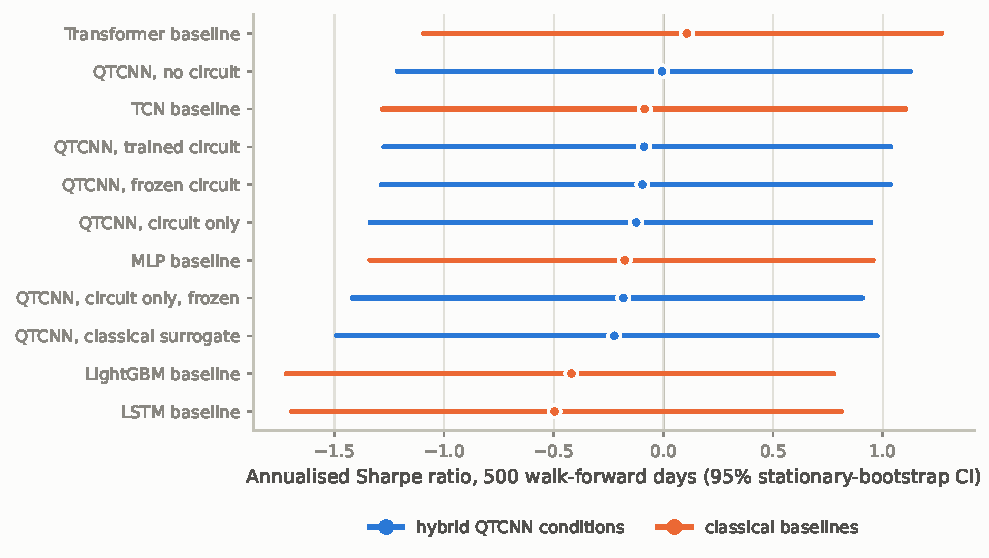
\includegraphics[width=\linewidth]{fig_ablation}
\caption{Annualised Sharpe ratio of each condition on the pooled 500-day
walk-forward track, with 95\% stationary-bootstrap confidence intervals. The
four hybrid conditions differ only in what occupies the quantum position.}
\label{fig:ablation}
\end{figure}

\begin{table}[t]
\centering
\caption{Out-of-sample performance on the pooled walk-forward track (\num{500} trading days, five seeds per condition). Confidence intervals are 95\% stationary bootstrap; DSR is the Deflated Sharpe Ratio deflated by the \num{55} configurations evaluated.}
\label{tab:headline}
\small
\begin{tabular}{lrrrrrr}
\toprule
Condition & Sharpe & 95\% CI & $p$ & DSR & Seed sd & Max DD \\
\midrule
Transformer baseline & +0.107 & [-1.09, +1.27] & 0.85 & 0.17 & 0.31 & -0.128 \\
QTCNN, no circuit & -0.006 & [-1.21, +1.13] & 0.99 & 0.14 & 0.20 & -0.164 \\
TCN baseline & -0.085 & [-1.28, +1.11] & 0.88 & 0.12 & 0.47 & -0.163 \\
QTCNN, trained circuit & -0.088 & [-1.27, +1.04] & 0.87 & 0.11 & 0.14 & -0.176 \\
QTCNN, frozen circuit & -0.096 & [-1.29, +1.03] & 0.86 & 0.11 & 0.15 & -0.178 \\
QTCNN, circuit only & -0.124 & [-1.34, +0.95] & 0.82 & 0.11 & 0.22 & -0.148 \\
MLP baseline & -0.176 & [-1.34, +0.96] & 0.74 & 0.09 & 0.61 & -0.116 \\
QTCNN, circuit only, frozen & -0.183 & [-1.42, +0.91] & 0.74 & 0.09 & 0.26 & -0.159 \\
QTCNN, classical surrogate & -0.224 & [-1.49, +0.97] & 0.71 & 0.08 & 0.35 & -0.192 \\
LightGBM baseline & -0.419 & [-1.72, +0.78] & 0.51 & 0.05 & 0.38 & -0.135 \\
LSTM baseline & -0.496 & [-1.69, +0.81] & 0.44 & 0.04 & 0.13 & -0.233 \\
\bottomrule
\end{tabular}
\end{table}


Nor is any condition distinguishable from the \textsc{None} control, the same
network with the circuit removed. Diebold--Mariano tests on the aligned daily
return series give $p = 0.66$ for \textsc{Trained}, \num{0.66} for
\textsc{Frozen}, \num{0.79} for \textsc{Surrogate} and \num{0.40} for the TCN
baseline; after Romano--Wolf stepdown correction the adjusted $p$ for every hybrid
contrast is \num{0.94}, and the smallest in the family of nine is \num{0.59}
(the circuit-only condition).

The fifth condition bounds the question from the other side. \textsc{QuantumOnly},
whose head sees the circuit output and nothing else, reaches a pooled Sharpe
ratio of \num{-0.251} (95\% CI $[-1.50, +0.85]$, $p = 0.65$) and an information
coefficient of \num{0.0058} ($t = 0.78$), identical to the no-circuit
control's ranking skill to the precision printed (Table~\ref{tab:ic}). It sits
\num{0.26} Sharpe below that control, with a paired standard error of
\num{0.26} ($p = 0.27$; Diebold--Mariano $p = 0.16$, Romano--Wolf $p = 0.56$).
The one-dimensional observable therefore ranks the cross-section as well as
the full hybrid network does, which on this task is barely at all, and placing
the encoder's features beside it recovers the no-circuit level rather than
exceeding it.

The gradient-boosted baseline does not change the picture. LightGBM on the
flattened window reaches a pooled Sharpe ratio of \num{-0.42} (95\% CI
$[-1.72, +0.78]$, $p = 0.51$), an information coefficient of \num{0.0051}
($t = 1.01$) and a turnover of \SI{72}{\percent} per leg per day, the highest
of the ten conditions; early stopping keeps \num{14} trees on average. It sits
\num{0.43} Sharpe below the no-circuit control ($p = 0.20$; Diebold--Mariano
$p = 0.37$). Whatever signal these features carry, the model family that wins
this competition on them extracts no more of it than the networks do.

The sharpest result is Figure~\ref{fig:trained-frozen}, and it is the one
contrast this design can resolve. A non-significant difference is not evidence
of no difference, so we state it as an equivalence rather than as a failure to
reject. On the pooled track the trained circuit and the same circuit frozen at
its initialisation differ by \num{-0.0008} in annualised Sharpe ratio, with a
paired stationary-bootstrap standard error of \num{0.0072}. Two one-sided
tests against a margin of \num{0.03} Sharpe give $p < \num{0.001}$: the
difference is inside that margin, not merely indistinguishable from zero. The
design could have detected a true difference of \num{0.02} at \SI{80}{\percent}
power, so the margin is not an artefact of a blunt instrument. Across the
twenty (fold, seed) cells the two agree to a correlation of \num{1.000}, their
information coefficients never differ by more than $5.5\times10^{-5}$, and their
validation AUCs by more than $3.9\times10^{-5}$.

The contrasts against the no-circuit control are weaker and we report them as
such. Because the study ranks by Sharpe ratio, these are tested twice: by a
Diebold--Mariano statistic on the difference of daily returns, which is a
hypothesis about means, and by a paired bootstrap on the difference of Sharpe
ratios, which is the hypothesis the table is ordered on. The two agree here,
with no contrast significant under either. The trained circuit beats that control by \num{-0.085} Sharpe with a
standard error of \num{0.239}; equivalence holds at a margin of \num{0.50}
($p = \num{0.03}$) but not at \num{0.25} ($p = \num{0.25}$), and the minimum
detectable effect at \SI{80}{\percent} power is \num{0.67}. The honest
statement is therefore that the circuit contributes less than half a Sharpe
unit, not that it contributes nothing. What is established is the narrower and
more diagnostic claim: optimising the circuit's eighteen parameters changes
nothing that freezing them does not change identically, so on this task the
quantum layer acts as a fixed random feature.

This is not simply a failure to train. The circuit does move. Instrumenting the optimiser over a fold, the eighteen
parameters travel an $L_2$ distance of \num{0.044} and \num{0.073} from
initialisations of norm \num{0.416} and \num{0.622}, that is by \SI{11}{\percent}
of their own magnitude. They move, and nothing downstream registers it: the
validation AUC of the trained and frozen conditions differ by at most
$3.9\times10^{-5}$. Whatever the circuit learns, the encoder and head absorb. This is
the behaviour \citet{bermejo2024quantum} predict for a randomly initialised
quantum convolutional network, which they show acts only on low-bodyness
information about its input and is reproduced by a classical surrogate built
from Pauli propagation. Their demonstration is on physics benchmarks; ours is
the same prediction measured on a financial ranking task, and it is
corroborated here by a surrogate that is not merely competitive with the
circuit but statistically equivalent to the network that has no circuit at
all.

Nor is it an artefact of the training budget. Early stopping halts the
walk-forward runs after \num{9.9} epochs on average, so a sceptic could hold
that the circuit was never given time to matter. Re-running both circuit
conditions for the full \num{30} epochs with early stopping disabled moves the
eighteen parameters further, by \SI{26}{\percent} of their initial norm on
average over the twenty cells (range \numrange{3}{70}\,\si{\percent}), and changes
nothing downstream: validation AUC \num{0.5133} for both conditions, differing
by at most $1.4\times10^{-4}$; information coefficients differing by at most
$5.9\times10^{-5}$; per-cell Sharpe ratios correlated at \num{0.999}; a pooled
difference of \num{-0.006} with a paired standard error of \num{0.009}, inside
the \num{0.03} margin ($p = 0.009$, minimum detectable effect \num{0.025}).
The longer budget lowers both conditions equally, from \num{-0.07} to
\num{-0.17} Sharpe, a mild overfitting the pair shares rather than a
contribution of the circuit.

The ordering survives a change of ansatz; the precision does not, and we
report both (Table~\ref{tab:reup}). On the re-uploading circuit with a ring of
entanglers and a global observable (Section~\ref{sec:method:arch}), the
trained and frozen conditions again sit below the no-circuit control, by
\num{0.24} and \num{0.20} Sharpe ($p = 0.45$ and \num{0.58}; Diebold--Mariano
$p = 0.37$ and \num{0.53}), their validation AUCs agree to $1.5\times10^{-4}$, their
per-cell Sharpe ratios correlate at \num{0.998}, and training moves the
\num{48} parameters by \SI{21}{\percent} of their initial norm. Two things
differ from the QCNN. The two conditions are no longer bit-for-bit alike:
information coefficients differ by up to \num{0.011} in a cell, where the QCNN
pair differed by $5.5\times10^{-5}$, so the global observable does let the
parameters reach the score. And the paired standard error of the pooled
Sharpe difference is \num{0.091}, twelve times the QCNN's, so two one-sided
tests certify equivalence only inside a margin of \num{0.25} ($p = 0.005$;
minimum detectable effect \num{0.25}) and not inside \num{0.03}
($p = 0.52$). The difference itself is \num{-0.032}, in the frozen circuit's
favour. What transfers across the two families is therefore the claim that
optimising the circuit does not improve on freezing it; the claim that it
changes nothing at all, to \num{0.03} Sharpe, is established for the QCNN
and bounded at \num{0.25} for the second family.

\begin{table}[t]
  \centering
  \caption{Second ansatz family (data re-uploading, CNOT ring, mean of $Z$
  over all wires) on the Tokyo walk-forward track, \num{500} days, five
  seeds; the no-circuit control is the one of Table~\ref{tab:headline}.
  Bootstrap 95\% intervals and $p$ against zero; information coefficient with
  its Newey--West $t$; $\Delta$ is the pooled Sharpe difference from the row
  above it with its paired standard error; TOST gives the smallest of the
  margins \num{0.03}, \num{0.10}, \num{0.25} at which equivalence holds at
  \SI{5}{\percent}.}
  \label{tab:reup}
  \small
  \begin{tabular}{lrcrrrr}
    \toprule
    Condition & Sharpe & 95\% CI & $p$ & IC ($t$) & $\Delta$ (s.e.) & TOST \\
    \midrule
    No circuit     & $+0.013$ & [$-1.14$, $+1.18$] & 0.99 & 0.0058 (0.88) & -- & -- \\
    Frozen circuit & $-0.190$ & [$-1.48$, $+0.97$] & 0.75 & 0.0084 (1.04) & $-0.203$ (0.389) & -- \\
    Trained circuit& $-0.222$ & [$-1.48$, $+0.95$] & 0.71 & 0.0077 (0.97) & $-0.032$ (0.091) & 0.25 \\
    \bottomrule
  \end{tabular}
\end{table}

\begin{figure}[t]
\centering
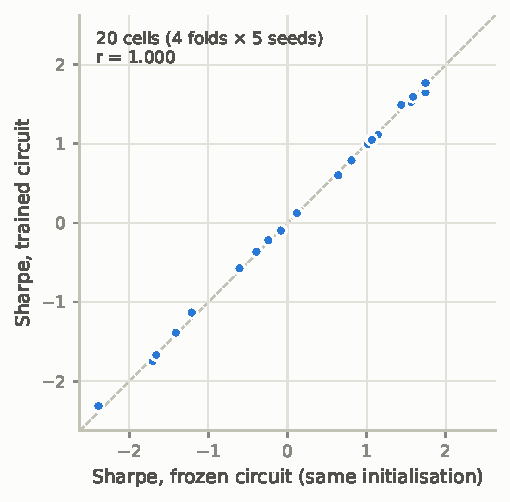
\includegraphics[width=0.55\linewidth]{fig_trained_vs_frozen}
\caption{Per-cell Sharpe ratio, trained circuit against frozen circuit. The
dashed line is the identity.}
\label{fig:trained-frozen}
\end{figure}

\subsection{Ranking skill}
\label{sec:results:ic}

Sharpe ratios are the metric this study is ordered on, but they confound a
model's ranking skill with the portfolio rule applied to it, and the nearest
prior work on the equity cross-section states its headline contrast as a
difference in information coefficient \citep{shen2026quantum}. We therefore
report the ranking statistics directly (Table~\ref{tab:ic}).

\begin{table}[t]
  \centering
  \caption{Ranking skill on both panels: the mean daily information
  coefficient, its Newey--West $t$-statistic, and the Spearman correlation
  between score decile and realised mean forward return as a monotonicity
  measure. Means over the twenty (JPX) and twenty-five (US) cells per condition.}
  \label{tab:ic}
  \small
  \begin{tabular}{lrrrrrr}
    \toprule
    & \multicolumn{3}{c}{JPX} & \multicolumn{3}{c}{US} \\
    \cmidrule(lr){2-4}\cmidrule(lr){5-7}
    Condition & IC & $t_{\mathrm{IC}}$ & Mono. & IC & $t_{\mathrm{IC}}$ & Mono. \\
    \midrule
    QTCNN, trained circuit     & 0.0069 &  0.96 &  0.144 & 0.0020 &  0.08 & -0.369 \\
    QTCNN, frozen circuit      & 0.0070 &  0.96 &  0.144 & 0.0020 &  0.08 & -0.386 \\
    QTCNN, classical surrogate & 0.0066 &  0.87 &  0.177 & 0.0039 &  0.29 & -0.298 \\
    QTCNN, no circuit          & 0.0058 &  0.88 &  0.127 & 0.0029 &  0.25 & -0.324 \\
    QTCNN, circuit only        & 0.0058 &  0.78 &  0.096 &   --   &   --  &   --   \\
    LightGBM baseline          & 0.0051 &  1.01 &  0.032 & 0.0034 &  0.50 & -0.149 \\
    TCN baseline               & 0.0054 &  0.73 &  0.021 & 0.0047 &  0.35 & -0.287 \\
    LSTM baseline              & 0.0058 &  0.75 & -0.042 & 0.0068 &  0.64 & -0.131 \\
    Transformer baseline       & 0.0060 &  0.77 & -0.046 & 0.0097 &  0.94 & -0.038 \\
    MLP baseline               & 0.0048 &  0.78 &  0.094 & 0.0027 &  0.30 & -0.191 \\
    \bottomrule
  \end{tabular}
\end{table}

Three readings, and the first is the one that matters for the ablation. The
trained and frozen circuits agree on every ranking statistic to the precision
printed: identical information coefficients to four decimal places, identical
$t$-statistics, identical monotonicity. The equivalence of
Section~\ref{sec:results:ablation} is therefore not an artefact of the
portfolio rule washing out a difference in the scores; the scores themselves
are the same.

Second, the effect sizes place this study where it belongs in the literature.
The largest difference in information coefficient between any hybrid condition
and the no-circuit control is \num{0.0012} on JPX, against the
\num{0.005} that \citet{shen2026quantum} report as an indistinguishable
kernel-swap contrast on Chinese A-shares, and no $t$-statistic on either panel
reaches \num{1}. Nothing here is a large effect measured imprecisely; the
effects are small.

Third, ranking skill does not translate into realised Sharpe, and on the US
panel it is actively misleading. Every condition has a positive mean
information coefficient there while every condition loses money, and every
decile monotonicity is negative --- the score orders the cross-section in the
direction opposite to realised returns at the extremes, which is where a
long--short book trades. The same dissociation, in the other direction, is what
Section~\ref{sec:results:reeval} finds in the reference implementation, whose
best-performing model has the worst information coefficient of nine. A paper
reporting only one of these two families of statistic can reach either
conclusion it prefers.

\subsection{What does vary}
\label{sec:results:seeds}

Figure~\ref{fig:seeds} shows why single-seed comparisons of these models cannot
be trusted. The seed controls only which \num{60000} of roughly \num{190000}
labelled training sequences a fold draws, yet within a fold the spread across
seeds (standard deviation \numrange{0.12}{1.70} in Sharpe units, and up to
\num{4.39} between the best and worst seed of one condition) exceeds every
between-condition difference in Table~\ref{tab:headline}. Fold 2, which covers
the 2020 recovery, is negative in \num{47} of its \num{50} cells; fold 3 is
positive in almost all of its. On this task the training draw and the test regime
matter, and the architecture does not.

\begin{figure}[t]
\centering
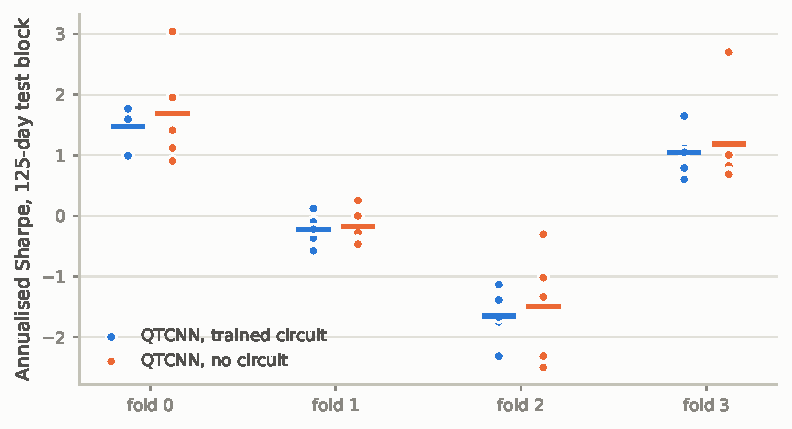
\includegraphics[width=0.9\linewidth]{fig_seed_spread}
\caption{Sharpe ratio per 125-day test block, one point per seed, for the
trained-circuit model and the no-circuit control. Bars mark seed means.}
\label{fig:seeds}
\end{figure}

The combinatorially symmetric cross-validation estimate of the probability of
backtest overfitting across the ten conditions is \num{0.67}: choosing the
in-sample best of them lands below the out-of-sample median in two
partitions out of three, worse than choosing at random.

\subsection{Transaction costs}
\label{sec:results:costs}

Turnover runs from \SI{34}{\percent} (LSTM) to \SI{72}{\percent} (LightGBM) of
each leg per day, and from \SI{49}{\percent} to \SI{54}{\percent} across the
five hybrid conditions. Figure~\ref{fig:cost} charges a round-trip cost on the
traded fraction of both legs. On the pooled track, break-even exists for
exactly one of the ten conditions, the no-circuit control at
\SI{0.06}{bps}, because the other nine have a negative gross mean return
before any cost is charged. Averaging the per-cell break-evens instead, as is
sometimes done, gives a far more flattering \numrange{2.8}{6.5}\,bps, but that
average is taken over only the nine to twelve cells in twenty whose gross
return was positive, and it is not comparable across conditions. At
\SI{5}{bps} the mean per-cell net Sharpe ratio runs from \num{-0.80} to
\num{-2.94}, and at \SI{10}{bps} from \num{-1.65} to \num{-5.63}. The reference implementation's own output, re-scored with the same procedure,
breaks even at \SI{7.4}{bps} on a turnover of \SI{24}{\percent}
(Section~\ref{sec:results:reeval}); neither figure describes a strategy that
could be traded.

\begin{figure}[t]
\centering
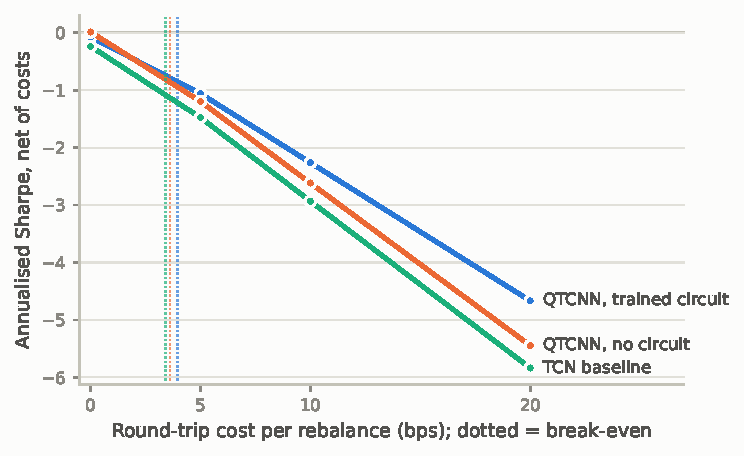
\includegraphics[width=0.75\linewidth]{fig_cost}
\caption{Annualised Sharpe net of round-trip transaction costs. Net Sharpe is
linear in cost at fixed turnover; dotted verticals mark break-even.}
\label{fig:cost}
\end{figure}

\subsection{Is the quantum signal at least orthogonal?}
\label{sec:results:spanning}

A model that loses head-to-head can still earn a place in an ensemble if its
return is not spanned by the alternatives. It is not. Regressing the
trained-circuit model's daily return on the four neural baselines gives
$R^2 = 0.936$ with an annualised intercept of \num{+0.024} and
$t = 1.07$ ($p = 0.28$); regressing it on its own no-circuit twin alone gives
$R^2 = 0.939$ and $t = -0.48$. Pairwise return correlations with the
classical models run from \num{0.89} to \num{0.97}, and an equal-weight blend
with any of them remains negative.

\subsection{A second market}
\label{sec:results:us}

If the null is a property of the task rather than of one exchange, it should
reappear elsewhere. We repeat the entire protocol on the US panel of
Section~\ref{sec:data-us}: the same conditions (nine; the circuit-only
condition was run on Tokyo only), the same code path, the
same five seeds, five walk-forward folds giving \num{625} pooled out-of-sample
days. Table~\ref{tab:headline-us} reports the result.

\begin{table}[t]
\centering
\caption{Out-of-sample performance on the pooled walk-forward track for the US panel (\num{625} trading days, five seeds per condition). Confidence intervals are 95\% stationary bootstrap; DSR is the Deflated Sharpe Ratio deflated by the \num{55} configurations evaluated.}
\label{tab:headline-us}
\small
\begin{tabular}{lrrrrrr}
\toprule
Condition & Sharpe & 95\% CI & $p$ & DSR & Seed sd & Max DD \\
\midrule
LSTM baseline & -0.655 & [-1.83, +0.50] & 0.28 & 0.00 & 0.55 & -0.402 \\
LightGBM baseline & -0.672 & [-2.00, +0.58] & 0.32 & 0.00 & 0.32 & -0.229 \\
Transformer baseline & -1.158 & [-2.34, +0.09] & 0.09 & 0.00 & 0.42 & -0.503 \\
QTCNN, no circuit & -1.441 & [-2.75, -0.05] & 0.05 & 0.00 & 0.16 & -0.532 \\
QTCNN, frozen circuit & -1.463 & [-2.75, -0.09] & 0.05 & 0.00 & 0.23 & -0.535 \\
QTCNN, trained circuit & -1.464 & [-2.74, -0.09] & 0.04 & 0.00 & 0.22 & -0.535 \\
QTCNN, classical surrogate & -1.491 & [-2.79, -0.14] & 0.04 & 0.00 & 0.28 & -0.535 \\
MLP baseline & -1.563 & [-2.92, -0.17] & 0.04 & 0.00 & 0.46 & -0.481 \\
TCN baseline & -2.026 & [-3.38, -0.64] & 0.01 & 0.00 & 0.27 & -0.530 \\
\bottomrule
\end{tabular}
\end{table}


The equivalence replicates, and more tightly than in Tokyo. The trained and
frozen circuits differ by \num{-0.005} Sharpe with a paired standard error of
\num{0.0075}; two one-sided tests against a \num{0.03} margin give
$p = \num{0.0005}$, and the minimum detectable effect at \SI{80}{\percent}
power is \num{0.02}. Their per-cell Sharpe ratios correlate at \num{0.9992}
and their pooled daily returns at \num{0.9999}. Against the no-circuit
control the picture is again weaker: equivalence holds at a \num{0.50} margin
and not at \num{0.25}, with a minimum detectable effect of \num{0.41}. No
Diebold--Mariano contrast is significant, nor is any paired bootstrap test of
the Sharpe difference itself, and nothing survives the Romano--Wolf correction,
whose smallest adjusted $p$ is \num{0.17}, for the LightGBM baseline.

What changes is the sign and, unlike the walk-forward on Tokyo data, the level.
Every condition loses money over this window, which runs from March 2019 to
September 2021 and contains both the COVID crash and the 2021 reversal, and for
three of them --- both circuit conditions and the TCN baseline --- the loss is
itself significant at the \SI{5}{\percent} level. The gross mean return is
negative for all nine, so no condition has a break-even transaction cost at
all. The four hybrid conditions cluster between \num{-1.24}
and \num{-1.44} while the four classical baselines sit between \num{-0.67}
(LightGBM) and \num{-0.85}; the gap is not significant under any test we apply, but it runs
against the hybrid family rather than for it. The backtest-overfitting
probability is \num{0.31}.

We draw one negative lesson from this panel about our own first attempt at it.
The pairwise return correlations across the eight network conditions run from
\num{0.53} to \num{1.000}, not the near-unity we initially measured: that
figure came from a single contaminated security-day, described in
Section~\ref{sec:data-us}, and the inference we had drawn from it --- that the
conditions move as one because they track a single signal --- was an artefact
of the error rather than a finding. The equivalence between trained and frozen
survived the correction unchanged, because a shared bad day cancels in a paired
difference; every level statistic on the panel did not.

Taken with Section~\ref{sec:results:ablation}: in two markets, on different
calendars, with different signs of gross performance, optimising the circuit
changes nothing that freezing it does not change identically, to within a
margin of \num{0.03} Sharpe that the design is powered to resolve.

\subsection{Re-evaluating the reference implementation}
\label{sec:results:reeval}

Contribution~4 is an audit, and an audit that only asserts is worth little. We
therefore re-scored the reference implementation's own saved predictions with
the procedure of Section~\ref{sec:protocol}, over the longest out-of-sample
window its outputs support --- \num{241} trading days rather than the \num{22}
it reported --- leaving its models, features and training untouched.
Table~\ref{tab:reeval} is the result.

\begin{table}[t]
  \centering
  \caption{The reference implementation's nine models, re-scored on
  \num{241} out-of-sample days (2020-12-10 to 2021-12-03) with annualised
  metrics, \SI{95}{\percent} stationary-bootstrap intervals, Deflated Sharpe
  Ratios and Newey--West information-coefficient $t$-statistics. Break-even is
  omitted where the gross return is not positive. Nothing else about the
  pipeline was changed.}
  \label{tab:reeval}
  \small
  \begin{tabular}{lrcrrrrr}
    \toprule
    Model & Sharpe & 95\% CI & $p$ & DSR & IC & $t_{\mathrm{IC}}$ & B/E (bps) \\
    \midrule
    QTCNN (reference)  &  1.80 & [-0.03,  3.79] & 0.07 & 0.54 & 0.0016 &  0.42 & 7.4 \\
    Transformer        &  0.46 & [-0.88,  2.04] & 0.53 & 0.11 & 0.0025 &  0.65 & 2.7 \\
    QLSTM              &  0.13 & [-1.42,  1.75] & 0.85 & 0.06 & 0.0132 &  2.37 & 0.8 \\
    LightGBM ranker    & -0.32 & [-2.34,  1.51] & 0.78 & 0.02 & 0.0060 &  1.52 & --  \\
    QNN                & -0.43 & [-2.31,  1.42] & 0.66 & 0.02 & 0.0148 &  2.10 & --  \\
    MLP                & -0.56 & [-2.24,  1.39] & 0.60 & 0.01 & 0.0134 &  2.57 & --  \\
    LSTM               & -0.59 & [-2.31,  1.27] & 0.49 & 0.01 & 0.0030 &  1.05 & --  \\
    PQC + LightGBM     & -0.76 & [-2.38,  1.06] & 0.39 & 0.01 & 0.0064 &  2.21 & --  \\
    QCNN-LSTM          & -2.15 & [-4.22, -0.17] & 0.04 & 0.00 & 0.0018 &  0.70 & --  \\
    \bottomrule
  \end{tabular}
\end{table}

Three things follow, and none of them requires disagreeing with the reference
implementation about anything except how it was scored.

First, the headline survives the longer window in point estimate but not in
inference. The quantum model is still ranked first, at an annualised Sharpe
ratio of \num{1.80}, but its bootstrap interval spans zero, its $p$-value is
\num{0.07}, and its Deflated Sharpe Ratio is \num{0.54} against the \num{0.95}
a claim requires. Eleven-fold more out-of-sample data does not convert the
result into a significant one; it reveals that the original window was too
short to tell.

Second, and more diagnostically, the ranking by Sharpe ratio and the ranking by
information coefficient are close to opposed. The quantum model has the
\emph{lowest} information coefficient of the nine (\num{0.0016},
$t = \num{0.42}$), while the three models whose information coefficients are
individually significant --- MLP at $t = \num{2.57}$, PQC\,+\,LightGBM at
\num{2.21}, QNN at \num{2.10} --- all have negative Sharpe ratios. A model that
ranks the cross-section better than its rivals and earns less from it is not
being rewarded for its ranking. On a \num{22}-day window that pattern is
invisible; over \num{241} days it is the most informative thing in the table.

Third, costs decide the rest. The reference model turns over \SI{24}{\percent}
of each leg per day and breaks even at \SI{7.4}{bps}; three of the nine have a
break-even at all, and the best of those is under \SI{8}{bps}. None of the nine
describes a strategy that could be traded at institutional costs, which is a
statement about the task and not about any of the architectures in it.

\subsection{Circuit-level diagnostics}
\label{sec:results:diagnostics}

The negative result above is not explained by the circuit being untrainable.
Figure~\ref{fig:barren} plots the variance of a circuit parameter's gradient at
random initialisation from two to twelve qubits: it moves from
$3.1\times10^{-3}$ to $2.0\times10^{-3}$, a fitted log-variance slope of \num{-0.036}
per qubit against the \num{-0.69} an exponential $2^{-n}$ decay would give.
The shared-parameter construction keeps the parameter count at $6L$ regardless
of width, and the measured observable is local, which are the conditions under
which barren plateaus are avoided. Expressibility, measured as KL divergence
from the Haar fidelity distribution, falls from \num{0.188} to \num{0.078}
between one and three layers at eight qubits, so the circuit is neither
degenerate nor flat. It is trainable; training it simply does not help.

\begin{figure}[t]
\centering
\begin{subfigure}[t]{0.48\linewidth}
  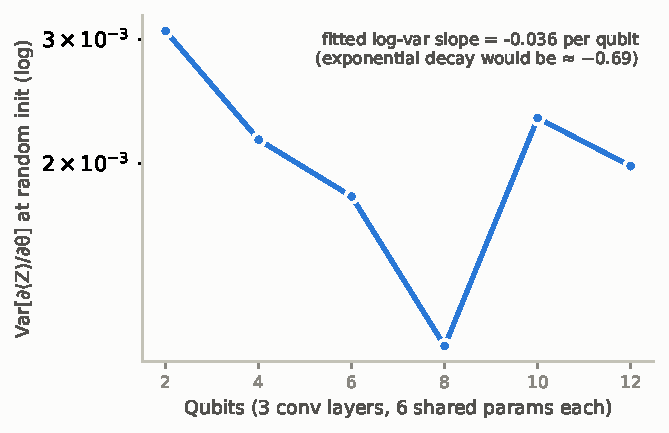
\includegraphics[width=\linewidth]{fig_barren}
  \caption{Gradient variance against register width.}
  \label{fig:barren}
\end{subfigure}\hfill
\begin{subfigure}[t]{0.48\linewidth}
  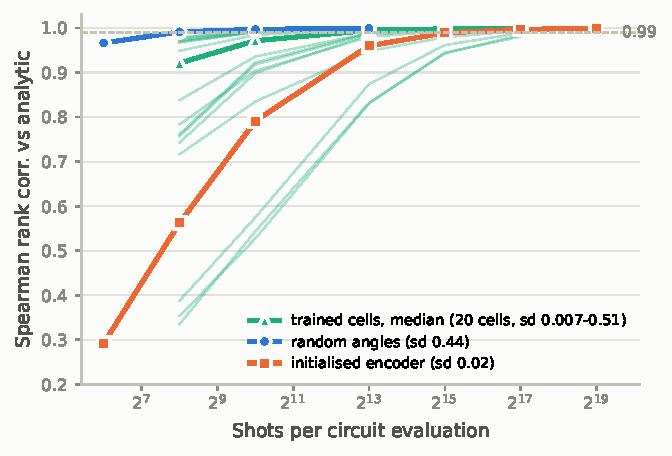
\includegraphics[width=\linewidth]{fig_shots}
  \caption{Rank preservation against shot budget, at both input
  distributions.}
  \label{fig:shots}
\end{subfigure}
\caption{Circuit-level diagnostics at eight qubits and three layers.}
\end{figure}

Figure~\ref{fig:shots} addresses deployment, and it is the one diagnostic in
this section whose answer depends on where the circuit's inputs come from. The
strategy consumes a ranking, so the relevant quantity is the Spearman
correlation between finite-shot and analytic scores within a trading date. On
the uniform random angles a circuit-level scan naturally uses, that correlation
is \num{0.991} at \num{256} shots and \num{0.9996} at \num{8192}, and the
implied budget is undemanding.

Those inputs are not the ones the model produces. Pushing real feature windows
through the encoder and measuring the spread of the circuit output
\emph{within} a cross-section gives a standard deviation of \num{0.018},
against \num{0.443} for random angles --- a factor of \num{24}. Shot
requirements scale with the spread of the quantities being ranked, and at the
real spread the same measurement gives a rank correlation of \num{0.56} at
\num{256} shots, \num{0.79} at \num{1024} and \num{0.96} at \num{8192}. Reaching
\num{0.99} takes about \num{32768} shots per security and reaching \num{0.997}
about \num{131072} (Table~\ref{tab:shots}). Scoring \num{2000} securities daily
therefore costs between $7\times10^{7}$ and $3\times10^{8}$ circuit executions
per trading day, two orders of magnitude above what the random-input scan
implies.

\begin{table}[t]
  \centering
  \caption{Rank preservation against shot budget, measured at two input
  distributions: uniform random angles, and the circuit inputs the encoder
  actually produces on real trading dates (12 dates, 300 securities each,
  within-date Spearman correlation against the analytic score).}
  \label{tab:shots}
  \small
  \begin{tabular}{rrr}
    \toprule
    Shots per security & Random angles (sd \num{0.443}) & Real cross-sections (sd \num{0.018}) \\
    \midrule
    64      & --      & 0.29 \\
    256     & 0.991   & 0.56 \\
    1\,024  & 0.997   & 0.79 \\
    8\,192  & 0.9996  & 0.96 \\
    32\,768 & --      & 0.989 \\
    131\,072& --      & 0.997 \\
    524\,288& --      & 0.9993 \\
    \bottomrule
  \end{tabular}
\end{table}

The mechanism is worth stating because it is a property of the task rather than
of the device. Cross-sectional normalisation and a trained encoder map a day's
securities into a narrow band of embedding angles, so the observable they
produce is concentrated; ranking within that band is a fine discrimination and
finite sampling resolves it slowly. Exponential concentration of quantum
observables is a known obstacle for kernels and reservoirs as system size
grows~\citep{miroszewski2024search}; what this measurement shows is a
task-induced version of it that is already severe at eight qubits, where the
system is far too small for the asymptotic argument to bite. A circuit-level
scan on random inputs cannot see it, which is a reason to measure shot budgets
on the deployed input distribution rather than a convenient one.

Gate noise, by contrast, is invisible at those budgets. Depolarising noise
scales a Pauli expectation by an input-independent factor, so it cannot reorder
scores; the rank correlation is \num{1.0000} at every rate up to $p = 0.05$
whether the rate is uniform across wires or drawn per wire. Under heterogeneous
depolarising noise at \num{1024} shots the correlation is \num{0.997} at
$p = 0$ and \num{0.997} at $p = 0.05$: sampling accounts for all of the
degradation. Amplitude damping, which is non-unital, produces a mean shift in
$\langle Z\rangle$ growing linearly to \num{0.026} at $\gamma = 0.05$ while
depolarising produces none --- confirming the measurement can distinguish the
two --- and still leaves the rank correlation above \num{0.9997}. For this
circuit and observable the deployment constraint is the sampling budget, not
device fidelity.

\subsection{Locked holdout}
\label{sec:results:holdout}

The supplemental window, 2021-12-06 to 2022-06-24 (\num{135} trading days),
was evaluated once per condition after that condition's design was frozen,
with each condition trained on all data to 2021-08-06 under the same validation
and embargo rules. It was opened for the eight network conditions, then for
the LightGBM baseline, and the eight network conditions were then re-run on it
under the released code because the first run could not be reproduced
(Section~\ref{sec:protocol:holdout}). Table~\ref{tab:holdout} reports the
reproducible run; Appendix~\ref{sec:app:rerun} gives the first.

\begin{table}[t]
\centering
\caption{Locked holdout, 135 trading days. Uncorrected
bootstrap $p$ against zero; Romano--Wolf $p$ across the eight contrasts with
the no-circuit control on this window (the two circuit-only
conditions and the second ansatz family were not); DSR deflated by the
\num{55} configurations (eleven models, five seeds) the study evaluated, using the
empirical dispersion of their Sharpe ratios on this window (sd \num{0.92},
expected maximum under the null \num{2.12}); break-even computed on the
pooled track, undefined where the gross return is not positive.}
\label{tab:holdout}
\small
\begin{tabular}{lrrrrrr}
\toprule
Condition & Sharpe & Seed sd & $p$ & $p_{\mathrm{RW}}$ & DSR & Break-even (bps) \\
\midrule
QTCNN, no circuit          & $+1.83$ & 0.84 & 0.07 & --   & 0.42 & 3.7 \\
QTCNN, classical surrogate & $+1.57$ & 1.08 & 0.18 & 0.95 & 0.34 & 5.5 \\
QTCNN, frozen circuit      & $+1.51$ & 1.05 & 0.17 & 0.95 & 0.33 & 4.4 \\
QTCNN, trained circuit     & $+1.49$ & 1.05 & 0.18 & 0.96 & 0.32 & 4.4 \\
TCN baseline               & $+1.37$ & 0.77 & 0.22 & 0.95 & 0.29 & 3.0 \\
Transformer baseline       & $+0.68$ & 0.87 & 0.47 & 0.54 & 0.15 & 2.1 \\
LSTM baseline              & $+0.67$ & 0.79 & 0.48 & 0.91 & 0.15 & 3.8 \\
LightGBM baseline          & $+0.49$ & 0.76 & 0.72 & 0.33 & 0.12 & 0.6 \\
MLP baseline               & $+0.42$ & 0.77 & 0.68 & 0.37 & 0.11 & 1.1 \\
\bottomrule
\end{tabular}
\end{table}

The window replicates the ablation and not the sign. Trained and frozen
circuits differ by \num{0.02}; the no-circuit control is the best of the four
hybrid conditions and the surrogate is no worse than either circuit; every
Diebold--Mariano contrast between a hybrid condition and the no-circuit control
has $p > 0.70$ (the classical baselines are closer, at \num{0.14} for LightGBM
and \num{0.16} for the MLP; one paired Sharpe-difference test, the MLP's,
reaches $p = 0.046$ uncorrected; none survives correction). Gross Sharpe
ratios are higher for all nine conditions than on the walk-forward track, which is a property of the
period, a stretch on which the cross-section rewarded the momentum and
liquidity features every model shares. The ranking of the nine is not stable
across the two windows: the transformer moves from first to sixth and the
no-circuit control from second to first, while the seed standard deviations
(\numrange{0.76}{1.08}) are wider than before because the window is short. What
is stable is the ablation itself (trained beside frozen, the surrogate no
worse than either, and no contrast significant), which is the quantity the
design was built to measure.

No condition is distinguishable from zero by the test on this window either.
For the best, the no-circuit control at \num{+1.83}, the percentile interval
just excludes zero ($[+0.02, +3.94]$) while the null-imposed bootstrap gives
$p = 0.07$, and its Deflated Sharpe Ratio is \num{0.42} against the
\num{0.95} a claim would require: deflated by the \num{55} configurations, the
expected maximum Sharpe under the null on \num{135} days is \num{2.12}, above
every row of the table. At \SI{5}{bps} one condition remains positive, the
surrogate at \num{+0.18}; at \SI{10}{bps} none do.


\section{Discussion}
\label{sec:discussion}

\subsection{What the ablation identifies}
The four hybrid conditions were designed so that their pairwise contrasts each
answer one question, and on this data every answer is the same.
\textsc{Trained} against \textsc{Frozen} asks whether optimising the circuit
matters: the per-cell Sharpe ratios correlate at \num{1.000}, so it does not.
\textsc{Frozen} against \textsc{Surrogate} asks whether the particular random
feature a quantum circuit computes differs from a classical one of equal
parameter count and matching output scale: on no panel can the two be told
apart, and the sign of the difference changes between panels. \textsc{Surrogate}
against \textsc{None} asks whether any extra scalar feature helps the head at
all: it does not. The circuit is a random feature, the random feature is not
special, and the head does not need it.

The same three contrasts give the same three answers on the US panel
(Section~\ref{sec:results:us}), where gross performance is negative rather than
positive. A result that survives a sign change in the underlying market is
about the layer, not about the window.

A null result on a task where nothing works might say little about the layer.
The locked holdout is the positive control for that concern. On those \num{135} days the shared signal is profitable for all
nine conditions, with gross annualised Sharpe ratios from \num{+0.42} (MLP)
to \num{+1.83} (the no-circuit control), and the ablation is unchanged there: trained beside frozen, the
surrogate no worse than either, and no contrast significant. The circuit adds
nothing in the regime where the features fail and nothing in the regime where
they work.

The result does not show that quantum convolutional layers are useless. It
concerns this task: daily cross-sectional ranking from twenty days of
technical features, where the achievable information coefficient is around
\num{0.006} and the spread of one model's Sharpe ratio across seeds
(standard deviation \numrange{0.13}{0.61}) is as large as the spread between
models (\num{0.17}). A layer cannot demonstrate value in a regime where the
signal it would need to improve on is itself indistinguishable from noise.

\subsection{Why earlier numbers looked different}
The reference study this work audits \citep{chen2025quantumb} reports an
out-of-sample Sharpe ratio of \num{0.538} $\pm$ \num{0.042} for its quantum
model, about \SI{72}{\percent} above its best classical baseline, and defines
that ratio as annualised. Its accompanying public implementation, which is the
artefact we re-ran, computes the ratio as mean over standard deviation with no
$\sqrt{252}$ factor and yields \num{0.33} on the same window; on the
conventional scale that is \num{5.2}. Whichever figure one takes, four things,
each individually sufficient, separate it from Table~\ref{tab:headline}. It
was computed on \num{22} trading days, a window over which the bootstrap
interval spans several Sharpe units in either direction; the authors
themselves note that \num{22} days give limited power and that about \num{45}
would be needed for \SI{90}{\percent} power, and defer a full-sample backtest
to future work. The headline is a single-seed model selection (noise
experiments use five runs), and the seed draw alone moves a fold's Sharpe by
up to \num{2.2} units for the two conditions in Figure~\ref{fig:seeds} and by
\num{4.39} for LightGBM. The split adjustment
ran forward in time, corrupting every momentum and volatility feature with
artefactual returns of up to \num{2300}\%. And the paper's own encoder-only
ablation already scores \num{0.412} $\pm$ \num{0.039}, so most of the reported
edge over the Transformer baseline is the temporal encoder, not the circuit, the same decomposition our \textsc{None} condition makes explicit. None of
these is exotic; all are common in the applied quantum machine learning
literature \citep{shen2026quantum,bowles2024better}, where evaluation practice
has not yet caught up with the standards of empirical finance.

\subsection{The circuit is trainable; that is not the problem}
The diagnostics rule out the explanation a quantum-computing reader would reach
for first. Gradient variance is flat from two to twelve qubits, so there is no
barren plateau; expressibility improves with depth, so the ansatz is not
degenerate; the rank of its outputs survives depolarising and amplitude-damping
noise at rates well above current hardware. The layer could be trained, and it
could be run. It has nothing to contribute here that the classical
encoder around it does not already provide.

\subsection{What a deployment would actually cost}
Because the strategy consumes a ranking, the operative hardware question is how
many shots preserve rank order at the spread of the scores being ranked, and
that spread is set by the trained model, not by the circuit. Across the twenty
trained cells the within-date standard deviation of the circuit output runs
from \num{0.007} to \num{0.51}, with a median of \num{0.10}, because
cross-sectional normalisation and the encoder map a day's securities into a
band of angles whose width the training trajectory decides. Preserving the
ranking to a Spearman correlation of \num{0.99} takes about \num{8192} shots
per security at the median cell, roughly $1.6\times10^{7}$ circuit executions
to score \num{2000} securities for one trading day, and more than
\num{131072} at the narrowest cells; the \num{256} a scan on random inputs
suggests is reached by no cell, and the widest need \num{1024}. Gate noise remains negligible at those budgets
(sampling accounts for essentially all of the degradation), so the cost is set
by measurement statistics alone.

We make no claim about whether a present device sustains that rate, and the
comparison that matters is not with a device specification but with the
classical alternative: the same ranking is produced by a parameter-matched
classical map in microseconds, and by no map at all equally well. The
conclusion is therefore narrower than the one a circuit-level scan would
support. It is not that hardware is no obstacle; it is that the obstacle is
mis-stated when the shot budget is measured on random inputs, or on one
encoder, and that on this task the observable can be concentrated enough to
make ranking expensive even at eight qubits, by an amount that varies a
hundredfold between statistically indistinguishable cells. Whether that
concentration is intrinsic to cross-sectional ranking or an artefact of this
encoder is the question we would put first in
any follow-up.

\subsection{Threats to validity}
\label{sec:discussion:threats}
We list the ways this study could be wrong, in decreasing order of how much
they would change the conclusion.

\paragraph{One feature set, chosen by us.}
All eleven conditions see the same \num{21} technical features. If the quantum
layer has an inductive bias suited to structure these features do not contain
(fundamentals, order-flow, cross-asset signals), the null is a statement
about the inputs rather than the layer. Nothing in the design can rule this
out, and it is the most likely way the result fails to generalise.

\paragraph{Two ansatz families, one of them resolved finely.}
The QCNN (angle embedding, shared two-qubit blocks, pooling, single-wire
measurement) and a re-uploading circuit with a CNOT ring and a readout
averaged over every wire give the same ordering, but only the first is certified equivalent
to its frozen copy inside \num{0.03} Sharpe; the second is bounded at
\num{0.25}, because its all-wire readout lets the parameters reach the
score and the paired standard error grows twelvefold. A family in which
training the circuit helps may exist; neither of these two is it, and the
second shows that a looser bound is what a more expressive circuit buys here.

\paragraph{Low achievable signal.}
The information coefficient available on this task is around \num{0.006}
(Table~\ref{tab:ic}), and the spread across seeds is as large as the
differences between conditions. A layer cannot demonstrate value where the signal
it would improve on is itself indistinguishable from noise. The locked holdout
is the partial answer: on a window where the shared signal does pay, the
ablation is unchanged. It is \num{135} days, which is short by this paper's own
standard. The gradient-boosted baseline is the other partial answer: the model
family that wins this competition extracts an information coefficient of
\num{0.005} from the same features, no more than the networks, so the weak
signal is a property of the inputs rather than of the architectures.

\paragraph{Statistical resolution.}
The design resolves the trained-versus-frozen contrast to a margin of
\num{0.03} Sharpe and the contrasts against the no-circuit control only to
\num{0.50}. The second of those is a weak bound and we do not claim more from
it. Four folds and five seeds give twenty paired cells, which is enough for the
first comparison and not for the others.

\paragraph{Simulation only.}
Every circuit result is from a state-vector simulator. The noise scans are
simulated channels, not device runs, and the shot analysis assumes independent
sampling. No claim here has been checked on hardware.

\paragraph{Survivorship in the auxiliary panels.}
The US universe comes from a current exchange symbol directory and excludes
firms delisted before it. A 2022--2025 extension of the JPX panel was also
assembled from the same source for a delisting audit; no result in this paper
uses it, because it is missing
\num{207} of the \num{2000} universe securities, of which the exchange's
official delisting lists account for all: \num{204} left through takeovers,
management buy-outs or squeeze-outs, one failed the listing-maintenance
standards, one was removed by the exchange and one delisted voluntarily. The
JPX development panel itself has the same character: its \num{2000} securities
are the competition's primary universe, fixed by the organiser at the end of
the training period (Section~\ref{sec:data}). All three universes are common
to every condition and to the earlier result we re-score, so the bias enters
no contrast, but absolute performance levels on any of them are not claimed. The US panel also
required a point-in-time price screen to remove a bankruptcy-reorganisation
splice (Section~\ref{sec:data-us}); we found it by auditing for impossible
returns, and a study that did not audit would not have found it.

\paragraph{Fold count.}
Four walk-forward folds are what the JPX sample supports; a fifth would need
\num{44} more trading days than exist. The US calendar affords five.

\subsection{What would change the conclusion}
A positive result would require a task where the circuit's inductive bias
matches structure in the data that the classical encoder cannot express. The
present data has no such structure to find: over the \num{500} development
days only one condition has a positive gross return, and a transaction cost of
half a basis point removes it; on the \num{135}-day holdout the best
break-even cost is \SI{5.5}{bps}. Claims of quantum
advantage in financial prediction should be accompanied by the control
conditions used here (a frozen circuit and a parameter-matched surrogate at
minimum) and by an evaluation long enough to resolve the effect being
claimed. Where they are, we expect most of them to look like
Table~\ref{tab:headline}.

\section{Conclusion}
\label{sec:conclusion}

We evaluated a hybrid quantum temporal convolutional network for daily
cross-sectional equity ranking under a protocol built to make the quantum
contribution identifiable: six conditions trained through one code path, four rolling-origin folds with an embargo, five seeds, annualised risk
metrics with bootstrap intervals, Deflated Sharpe Ratios, backtest-overfitting
probabilities and family-wise error control. On \num{500} out-of-sample
trading days the trained circuit is indistinguishable from the same circuit
frozen at initialisation, from a parameter-matched classical surrogate, and
from the network with the circuit removed; no condition is distinguishable from
zero, and ten of the eleven have no break-even transaction cost at all. Two
one-sided tests place the trained-versus-frozen difference inside \num{0.03}
annualised Sharpe in both markets, and inside \num{0.10} when the circuit is
trained to the full budget without early stopping, which is equivalence rather than a failure
to reject; the contrast against the no-circuit control is resolved only to
\num{0.50}.

The circuit is not the weak point. It has no barren plateau to twelve qubits,
and its output ranking is robust to gate noise; a second ansatz family, with
re-uploading and an observable read from every wire, reproduces the ordering and bounds its
trained-versus-frozen difference at \num{0.25} Sharpe. What is
expensive is measurement: at the spread the trained models produce on a real
cross-section, preserving the ranking takes about \num{8192} shots per
security at the median cell, and more than \num{131072} at the narrowest,
rather than the \num{256} a scan on random inputs suggests. The weak point is the task, on which the achievable signal is
smaller than the variance introduced by the training draw. Earlier reports of
advantage on this data came from a 22-day window, single-seed model selection,
a split adjustment applied in the wrong direction in the public implementation,
and a classical encoder that already accounts for most of the reported gain.

Two artefacts are released with the paper (\url{https://github.com/ChiShengChen/qtcnn-trained-frozen-absent}): a batched formulation of the quantum
convolutional layer that reproduces the per-sample implementation to
double precision at a \numrange{33}{72}-fold speed-up, and the evaluation stack itself,
calibrated on synthetic data with known answers. Both are reusable on any
cross-sectional ranking task. We hope the second is used more often than the
first.


\appendix
\section{Reproducibility}
\label{sec:repro}

\subsection{Software and hardware}
Experiments ran on a 24-core workstation shared with unrelated jobs, under
PennyLane 0.42.3, PyTorch 2.6.0, NumPy 1.26.4 and pandas 2.2.3 on Python
3.12.9. Quantum circuits were simulated on the \texttt{default.qubit}
state-vector backend with backpropagation. All reported models are trained on
CPU: for an eight-qubit register the simulator is CPU-bound, and a GPU gives no
benefit.

\paragraph{Measurement under contention.}
Wall-clock figures are sensitive to what else the machine is running. The same
training step measured \SI{16.4}{\second} at a one-minute load average of 57 on
24 cores and \SI{0.38}{\second} once the machine was scheduled, a factor of 43.
Every timing reported here was taken through a job scheduler that admits work
against declared CPU, RAM and VRAM, and the load at measurement time is
recorded alongside the figure.

\subsection{Determinism}
Each (model, fold, seed) cell seeds PyTorch, NumPy and the training-set
subsample from the same integer. Circuit parameters are initialised from a
dedicated generator so that the \textsc{Frozen} condition draws exactly the same
weights as the \textsc{Trained} condition's initialisation. Results are
checkpointed per cell, so an interrupted sweep resumes without recomputing
completed work and without changing any seed.

\subsection{Data and code}
The dataset is the public JPX Tokyo Stock Exchange
panel~\citep{jpx2022competition}. The analysis code, including the evaluation
statistics, the walk-forward protocol and the batched circuit, is released with
the paper. The calibration checks reported in
Section~\ref{sec:protocol:stats} --- in particular that the
backtest-overfitting estimator returns \num{0.53(4)} on independent random
strategies --- are part of the test suite.

\subsection{Deviations from the reference implementation}
The pipeline this work audits --- our own, as stated in
Section~\ref{sec:intro} --- differs in four respects that materially affect its
numbers, each corrected here: the split adjustment direction
(Section~\ref{sec:data:adjustment}); the Sharpe ratio, which the released code
computes as mean over standard deviation with no annualisation, though the
published paper states that its metric is annualised; the evaluation window,
which date subsampling reduced to \num{22} trading days; and the absence of
transaction costs. Section~\ref{sec:results:reeval} reports the original models
re-scored over \num{241} days with all four corrected, so that the difference
is attributable rather than asserted.


\section*{Declarations}

\subsection*{Availability of data and materials}
The JPX panel is the public competition dataset \citep{jpx2022competition} and
is not redistributed here. The United States panel is reconstructed from public
daily prices by the scripts released with this paper at
\url{https://github.com/ChiShengChen/qtcnn-trained-frozen-absent}, which also
contain the evaluation stack, the calibration tests, the per-cell results and
daily return series behind every table and figure in this manuscript, the
trained weights of the cells used for the shot-budget measurement, and the
legacy pipelines re-evaluated in Section~\ref{sec:results:reeval}.

\subsection*{Competing interests}
The reference implementation and published result re-examined in this paper are
the authors' own \citep{chen2025quantumb}. The authors declare that they have no
competing interests.

\subsection*{Funding}
EJK acknowledges financial support from the National Science and Technology
Council (NSTC) of Taiwan under Grant No.~NSTC~114-2112-M-A49-036-MY3.

\subsection*{Authors' contributions}
CSC designed the study, wrote the code, ran the experiments and drafted the
manuscript. EJK contributed to the analysis and interpretation of the quantum
diagnostics and revised the manuscript. Both authors read and approved the
final manuscript.

\subsection*{Acknowledgements}
Not applicable.

\bibliographystyle{plainnat}
\bibliography{refs,refs_generated}

\end{document}
